\documentclass{beamer}

\setbeamertemplate{footline}[frame number]

\usepackage{multimedia}

\usepackage{amsmath}
\usepackage{amsfonts}

\usepackage{graphicx}
\graphicspath{{data/}}

\usepackage{pgfplots}
\usepackage{tikz}
\usetikzlibrary{arrows, shapes, fit, decorations.markings}

\tikzstyle{vecArrow} = [thick, decoration={markings,mark=at position
   1 with {\arrow[semithick]{open triangle 60}}},
   double distance=1.4pt, shorten >= 5.5pt,
   preaction = {decorate},
   postaction = {draw,line width=1.4pt, white,shorten >= 4.5pt}]
\tikzstyle{innerWhite} = [semithick, white,line width=1.4pt, shorten >= 4.5pt]

\makeatletter
  \def\inputTikZ{\@ifnextchar[{\@with}{\@without}}
  \def\@with[#1]#2{
    \begingroup
      \tikzset{every picture/.style={scale=#1}}
      \input{data/#2.tikz}
    \endgroup
  }
  \def\@without#1{\input{data/#1.tikz}}
\makeatother

\newcommand{\TODO}[1]{\emph{\small{{\bf TODO: } #1}}}

\newcommand{\etal}{\textit{et al. }}
\newcommand{\etc}{\textit{etc. }}
\newcommand{\eg}{\textit{e.g. }}

\title{Multi-Sensory Integration : Theories, Observations and Neural Implementation}
\author{Weipeng He \\ \texttt{2he@informatik.uni-hamburg.de}}
\date{July 5, 2013}

\begin{document}

\frame{\titlepage}

\begin{frame}
\frametitle{Outline}
\tableofcontents
\end{frame}

\section{Introduction}
\begin{frame}
  \frametitle{Introduction}
  \begin{itemize}
    \item ``Multisensory integration'' is the process of combining sensory cues of different modality.
    \item Multi-modal senses provide complementary information.

    ~
    \item Examples:
    \begin{itemize}
      \item Visual-auditory integration for spatial localization.
      \item Visual-haptic integration for perceiving the size and position;
      \item Visual-vestibular integration for perceiving self-motion;
    \end{itemize}
  \end{itemize}
\end{frame}

\begin{frame}
  \frametitle{Ventriloquist effect}
  \begin{center}
    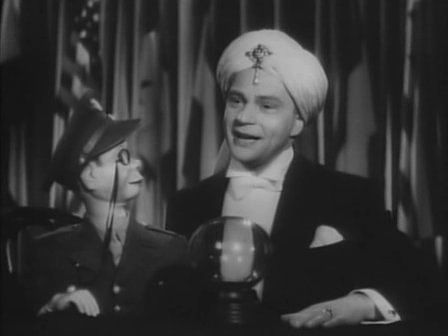
\includegraphics[width=.8\textwidth]{ventriloquism}
  \end{center}
\end{frame}

\begin{frame}
  \frametitle{Stream/bounce illusion}
  \begin{center}
    \movie[externalviewer=totem]{
\includegraphics[width=.6\textwidth]{streambounce}}{video/streambounce.mp4}
  \end{center}
\end{frame}

\begin{frame}
  \frametitle{Two major types of study}
  \begin{center}
    \inputTikZ[.9]{flow}
  \end{center}
  \begin{itemize}
    \item Psychophysics versus Neurophysiology.
    \item (Behavioral) versus (Neuronal).
    \item What can be done in the missing part?
  \end{itemize}
\end{frame}

\begin{frame}
  \frametitle{The end}
  \begin{center}
    \Huge{Thank you!}

    \Huge{Questions?}
  \end{center}
\end{frame}

\end{document}
